\documentclass{cekarticle}
\usepackage{color}
\usepackage{amsmath}
\usepackage{amssymb}
\usepackage{array}

\begin{document}

%=============================================================================
% Title page
%=============================================================================

\title{Systems Biology Markup Language (SBML) Level 2 Proposal: Array Features}

\author{Andrew Finney, Victoria Gor, Eric Mjolsness, Hamid Bolouri}

\authoremail{
\begin{minipage}{\textwidth}\centering
afinney@cds.caltech.edu, gor@aig.jpl.nasa.gov,\\Eric.D.Mjolsness@jpl.nasa.gov, hbolouri@cds.caltech.edu
\end{minipage}}

\maketitlepage

%=============================================================================
\section{Introduction}
\label{sec:introduction}
%=============================================================================

This document describes proposed features for inclusion in
Systems Biology Markup Language (SBML) Level 2. This document
describes features enabling the inclusion of arrays of processes,
structures or entities in models.  These features would allow a
model to be assembled from many copies of identical parts.  These
features enable the representation of patterns of connection
amongst array elements.

This document is not a definition of SBML Level 2 or part of it.
This document simply presents various features which could be
incorporated into SBML Level 2 as the Systems Biology community
wishes.  This document is intended for detailed review by that
community and to provoke alternative proposals.  Throughout this
document issues that the authors believe will require further
discussion have been highlighted.

For brevity the text of this document is with reference to SBML
Level 1~\citep{hucka:2001} i.e. features are described in terms
of changes to SBML Level 1.  This document uses UML diagrams in
the same way except that new features are shown in red.

All types proposed in this document will be derived from the
\texttt{SBase} type.

The features described in this document are built upon the
features defined in~\citet{finney:2002c}.

The appendix~\ref{sec:operators} lists all the SBML Level 1 operators
with all the operators proposed in this document.

\section{Models}

The proposed structure of the \texttt{Model} type is shown in
figure~\ref{fig:model}. A model would have optional lists of
\texttt{Domain} and \texttt{ArraySpecification} structures.

\begin{figure}[h]
  \vspace*{8pt}
  \centering
  
\includegraphics[scale = 0.7]{model}
  \caption{The definition of the Model type}
  \label{fig:model}
\end{figure}

\texttt{Domain} structures are described in
section~\ref{sec:domain} and \texttt{ArraySpecification}
structures are described in section~\ref{sec:arrayspec}.

\section{Domains}
\label{sec:domain}

In this proposal the bounds of an array are separated from an
actual array definition.  Array bounds are defined by these
proposed \texttt{Domain} structures, which are shown in UML form
in figure~\ref{fig:domain}.  A \texttt{Domain} structure consists
of a name (of \texttt{SName} type) and inclusive upper and lower
bounds of \texttt{int} type.  These bounds values can be
negative.  The upper bound must be greater than the lower bound.
We suggest that Domains exist in their own namespace i.e. a
domain name must unique among all the domains in the model but
can have the same name as another non-domain structure in the
model.

\begin{figure}[h]
  \vspace*{8pt}
  \centering
  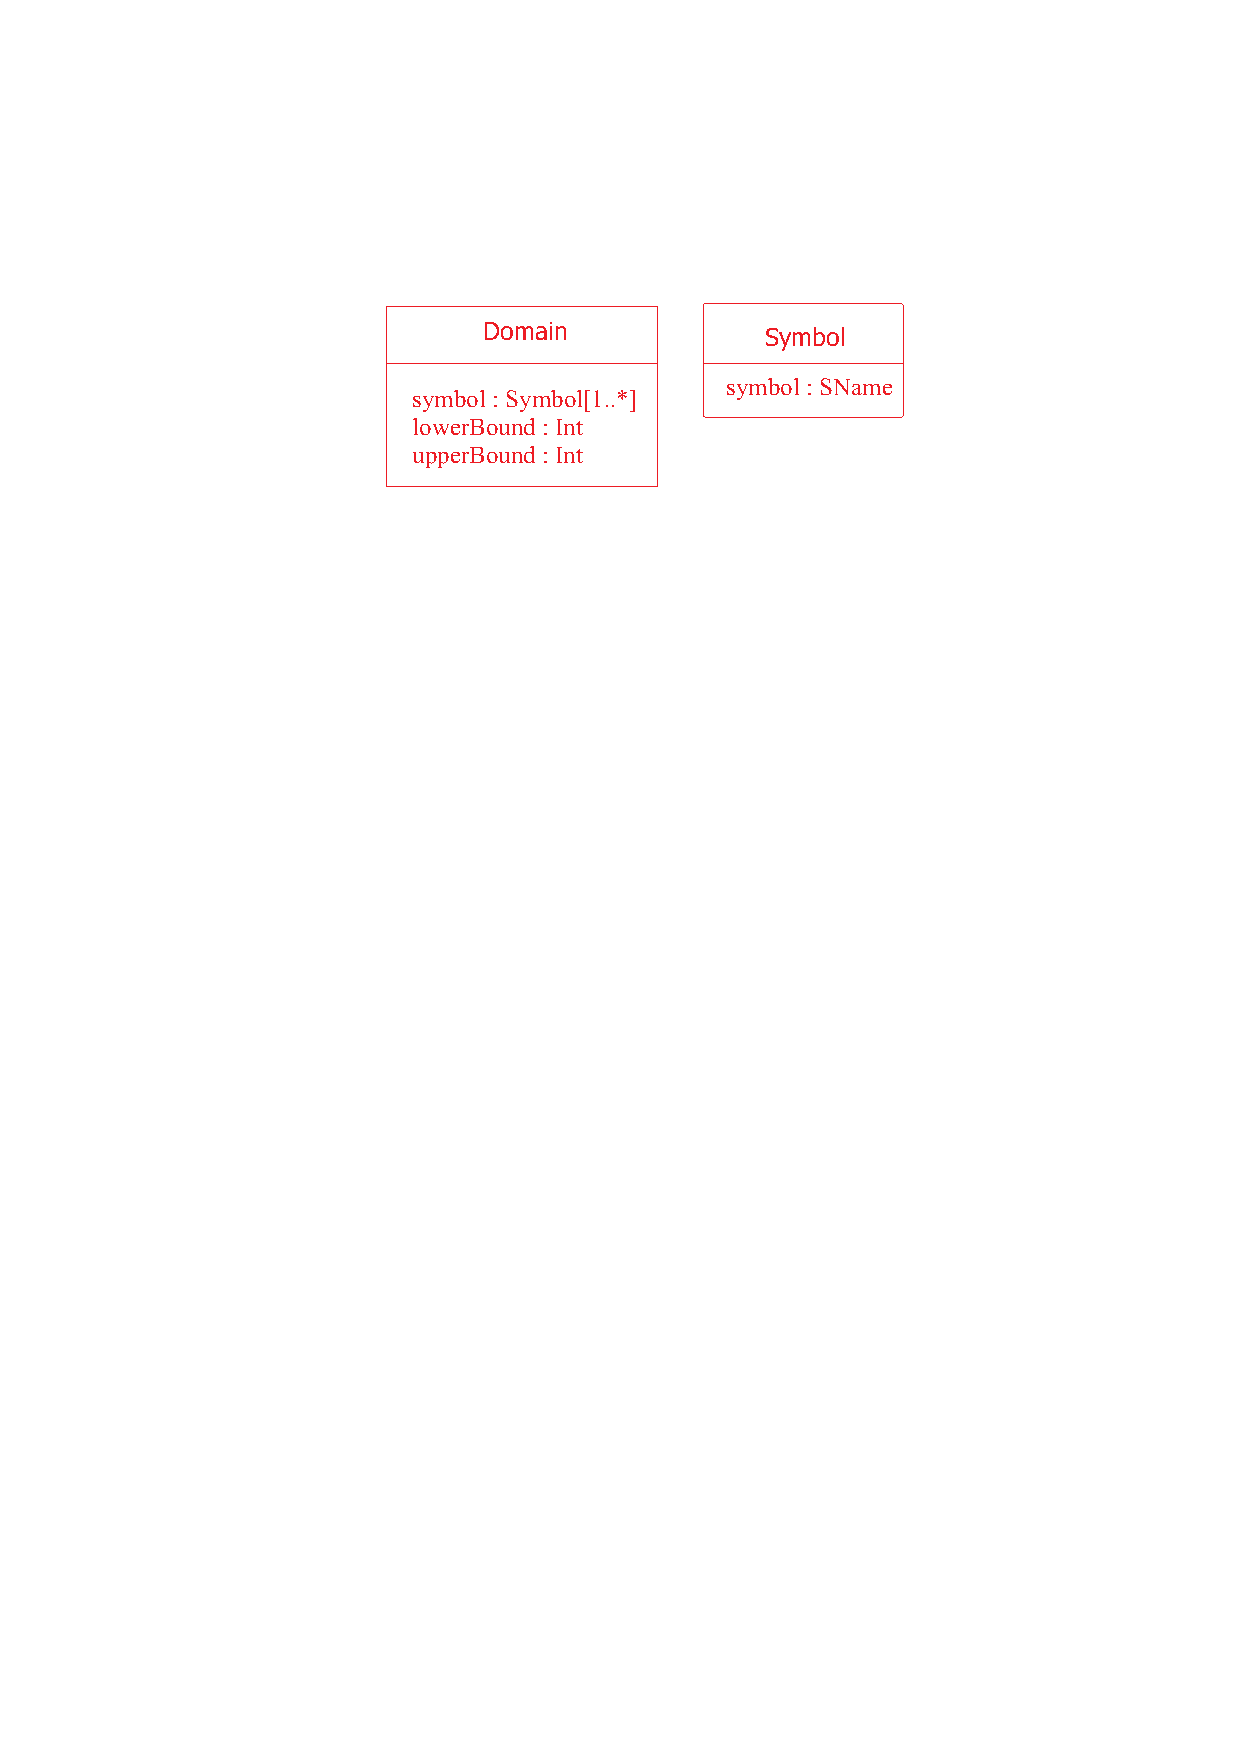
\includegraphics[scale = 0.7]{domain}
  \caption{The definition of the Domain type}
  \label{fig:domain}
\end{figure}

\subsection{Example}

The following example shows a \texttt{Model} structure
incorporating a \texttt{Domain} structure called \texttt{x} which
ranges from -10 through to 10.

\begin{example}
<model name="tissue">
    <listOfDomains>
        <domain name="x" upperBound="10" lowerbound="-10"/>
    </listOfDomains>
    ...
</model>
\end{example}

\section{Array Specifications}
\label{sec:arrayspec}

Within this proposal the next stage in defining an array is to
specify the array `shape' by specifying the number of dimensions
and assigning a domain to each dimension.  The proposed
\texttt{ArraySpecification} structure shown in UML form in
figure~\ref{fig:arrayspec} encapsulates this data.

\begin{figure}[h]
  \vspace*{8pt}
  \centering
  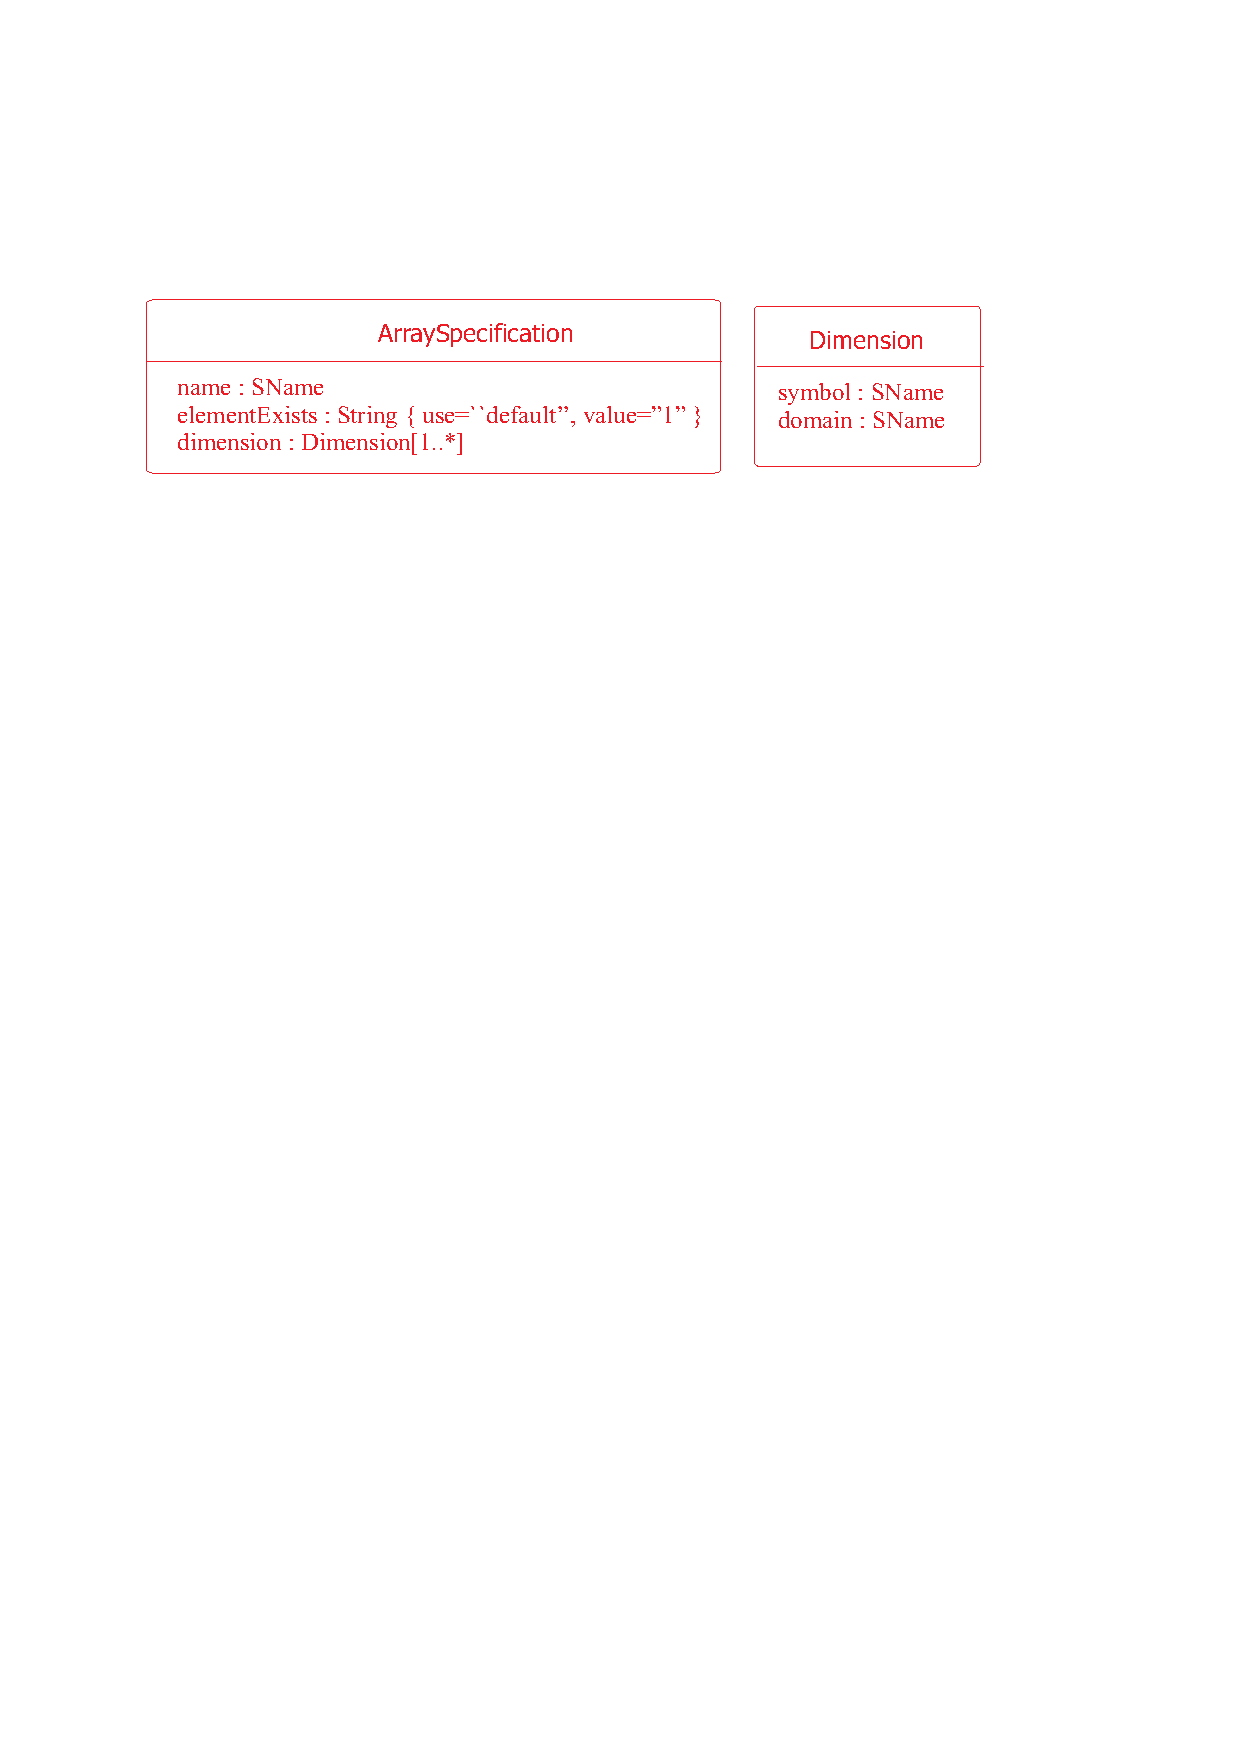
\includegraphics[scale = 0.7]{arrayspec}
  \caption{The definition of the ArraySpecification type}
  \label{fig:arrayspec}
\end{figure}

An \texttt{ArraySpecification} structure consists, in its
simplest form, of a name field, of type \texttt{SName}, and a list
of \texttt{Dimension} structures.  A \texttt{Dimension} structure
consists of a symbol field and a domain field, both of type
\texttt{SName}.  The domain field refers to a preceding
\texttt{Domain} structure.  The symbol field identifies the
\texttt{Dimension} structure.  The function of the symbol field will be
described in section~\ref{sec:constantExpressions}.

The arrays specified by a given \texttt{ArraySpecification}
structure will have a dimension for each enclosed
\texttt{Dimension} structure.  The bounds of each dimension are
defined by the \texttt{Domain} field referenced by the
\texttt{Dimension} structure.

We suggest that \texttt{ArraySpecification} structures exist in
their own namespace i.e. a \texttt{ArraySpecification} name must
unique among all the \texttt{ArraySpecification} structures in
the model but can have the same name as another
non-\texttt{ArraySpecification} structure in the model.

\subsection{Simple Array Specification Example}
\label{sec:simplearray}

The following example shows the specification for a 2 dimensional
array of 10 by 5 elements indexed from 0.

\begin{example}
<model name="tissue">
    <listOfDomains>
        <domain name="x" upperBound="9" lowerbound="0"/>
        <domain name="y" upperBound="4" lowerbound="0"/>
    </listOfDomains>
    <listOfArraySpecfications>
        <arraySpecification name="grid">
            <listOfDimensions>
                <dimension domain="x"/>
                <dimension domain="y"/>
            <listOfDimensions>
        </arraySpecification>
    </listOfArraySpecifications>
    ...
</model>
\end{example}

\section{Arrays}

The core of this proposal is the idea that almost all the
structures in SBML can be defined as arrays as well as single
named objects.  To this end, we propose that the following SBML
types have a new optional field \texttt{arraySpecification} of
type SName: \texttt{Specie}, \texttt{Compartment},
\texttt{Reaction}, \texttt{Parameter} and \texttt{Rule}.  The
\texttt{arraySpecificiation} field when present should contain
the name of an \texttt{ArraySpecification} structure.

The presence of an \texttt{arraySpecificiation} field on a
structure indicates that the structure represents an array of the
objects.  All the objects in the array have the properties
described by the structures's attributes and substructures. The
array shape is defined by the named \texttt{ArraySpecification}
structure.

Structures that have an \texttt{arraySpecificiation} field value
share the same namespace as those structures that represent
single objects.

\subsection{Simple Array Example}
\label{sec:simplearrayeg}

The following SBML fragment shows a \texttt{Compartment}
structure representing a 1 dimensional array.

\begin{example}
<model name="simple">
    <listOfDomains>
        <domain name="x" upperBound="9" lowerbound="0"/>
    </listOfDomains>
    <listOfArraySpecfications>
        <arraySpecification name="strip">
            <listOfDimensions>
                <dimension symbol="X" domain="x"/>
            </listOfDimensions>
        <arraySpecification>
    </listOfArraySpecifications>
    <listOfCompartments>
        <compartment name="cell" arraySpecification="strip"/>
    </listOfCompartments>
    ...
</model>
\end{example}

\subsection{Constant Symbols and Expressions}
\label{sec:constantExpressions}

The symbol field of a \texttt{Dimension} structure defines a
symbol which can be used in numeric expressions.  For each element
of an array the symbol is assigned the index value of the element.
Although these symbol values vary over a domain they are constant
for the duration of a simulation.  These symbols are called
\emph{constant symbols}. It is possible to create expressions
using these symbols. It is possible to distinguish between constant and
dynamic expressions: in a constant expression all operands and
function arguments are either \texttt{Dimension} symbols or a
constant numeric values.

Constant expressions can then be used in place of most constant
attribute values of type \texttt{double} throughout SBML.
Constant symbols can occur in any numeric expression, for example
a rate equation. As symbols given on \texttt{Dimension}
structures are used in expressions they share the same namespace
as other SBML structures such as species.

An examples of this feature is given in section ~\ref{sec:useconsts}.

\subsection{Using Constant Symbols}
\label{sec:useconsts}

The constant symbols defined in an array specification can be
used within any structure that references that array
specification.  For example we can
modify the example from section~\ref{sec:simplearrayeg}, to
enable each element of the compartment array to have a different
volume. The \texttt{Compartment} structure is changed from
\begin{example}
<compartment name="cell" arraySpecification="strip"/>
\end{example}
to
\begin{example}
<compartment name="cell" volume="1 + X/0.1" arraySpecification="strip"/>
\end{example}

Notice that although constant symbol \texttt{X} varies over the
domain \texttt{x} this variance only defines the structure of the
model so that \texttt{X} is not a parameter or variable of any
simulation of the model.

\subsection{Referencing Array Elements}

It is proposed that in place of a symbol for a single object it
is possible to refer to a element of an array.  This is achieved
by using the \texttt{[]} array operator, which is similar to the
C array operator.  In numeric expressions this operator is
syntactically equivalent to a function call. The array operator
can also be used in any field which refers to a \texttt{Specie},
\texttt{Compartment}, \texttt{Reaction}, \texttt{Parameter} or
\texttt{Rule} structure by name for example the \texttt{specie}
field on a \texttt{SpecieReference} structure can contain an
array operator instead of an \texttt{SName} type.

The `array' operand of an array operator must be the name of a
structure which has an \texttt{arraySpecification} field value.
We suggest that the index operand to an array operator be
restricted to being a constant expression.  An array operator
when applied to an array of consisting of $n$ dimensions results
in an array of $n-1$ dimensions and if $n$ is 1 then the result
is a single object. The order of application of the array
operator to array dimensions follows the order of the
\texttt{Dimension} structures as given on the corresponding array
specification.

We can extend the example shown in
section~\ref{sec:simplearrayeg} to include an array of species
placed in an array of compartments:
\begin{example}
<model name="simple">
    <listOfDomains>
        <domain name="x" upperBound="9" lowerbound="0"/>
    </listOfDomains>
    <listOfArraySpecfications>
        <arraySpecification name="strip">
            <listOfDimensions>
                <dimension symbol="X" domain="x"/>
            </listOfDimensions>
        <arraySpecification>
    </listOfArraySpecifications>
    <listOfCompartments>
        <compartment name="cell" arraySpecification="strip"/>
    </listOfCompartments>
    <listOfSpecies>
        <species
            name="s" arraySpecification="strip" compartment="cell[X]"/>
    </listOfSpecies>
    ...
</model>
\end{example}
In this example each species array element is placed in a
corresponding compartment.

\section{Sparse Arrays and Connections}

\subsection{Sparse Array Specifications}

In practice arrays are not very useful for modeling unless its
possible to describe connection schemes between elements of the
arrays.  For example if one creates a model of a tissue of cells
as an array of compartments then the model doesn't become
interesting until the interactions between the cells are
incorporated.  This section begins the process of proposing
structures which allow interconnection schemes to be defined.

In this proposal \texttt{ArraySpecification} structures include
an additional \texttt{elementExists} field, as shown in
figure~\ref{fig:arrayspec}.  This field contains a constant
expression which defines whether an element actually occurs at a
given position in the array specification.  This expression is
conditional, which means that a zero value (false) implies that
the element won't occur and a non-zero value (true) implies that
an element will occur (conditional expressions are described in
more detail in~\citet{finney:2002c}).

The symbols that can occur in the \texttt{elementExists}
expression are limited to built-in functions, functions defined
by \texttt{Function} structures, and constant symbols.

The default value of \texttt{elementExists}, 1, ensures that
by default the shape of the array specification is determined
as described in section~\ref{sec:simplearray}.

Apart from the \texttt{elementExists} field, constant
symbols only have values for those elements that exist in the
array specification in which they are declared.

The index operand to an array operator must refer to a an element
which exists in the array.  This means that the index must be
within the domain to which it is applied and, in the case of
sparse arrays be a value to which the \texttt{elementExists}
expression returns a non-zero value.

\subsection{Sparse Array Specification Example}
\label{sec:sparseeg}

The following example shows a proposed
\texttt{arraySpecification} structure for triangular arrays where
the maximum \texttt{y} index is equal to the \texttt{x} index.

\begin{example}
<model name="starfish">
    <listOfDomains>
        <domain name="X" upperBound="9" lowerbound="0"/>
        <domain name="Y" upperBound="9" lowerbound="0"/>
    </listOfDomains>
    <listOfArraySpecfications>
        <arraySpecification name="triangle" elementExists="y <= x">
            <listOfDimensions>
                <dimension symbol="x" domain="X"/>
                <dimension symbol="y" domain="Y"/>
            <listOfDimensions>
        </arraySpecification>
    </listOfArraySpecifications>
    ...
</model>
\end{example}

\subsection{Using Sparse Array Specifications to Represent Connection schemes}
\label{sec:connections}

We can use a proposed sparse array specification to present the
connections between elements of another array.  This is shown in
the following example, in which the specification, \texttt{grid},
defines a 2 dimensional array and the specification,
\texttt{connections} defines a sparse 4 dimensional array
representing connections between elements of \texttt{grid}.
\texttt{connections} contains adjacent array elements for all pairs of
co-ordinates (over the \texttt{x} and \texttt{y} domains) where
the co-ordinates are exactly one array element away from each other.

\begin{example}
<model name="tissue">
    <listOfDomains>
        <domain name="x" upperBound="9" lowerbound="0"/>
        <domain name="y" upperBound="4" lowerbound="0"/>
    </listOfDomains>
    <listOfArraySpecfications>
        <arraySpecification name="grid">
            <listOfDimensions>
                <dimension domain="x"/>
                <dimension domain="y"/>
            <listOfDimensions>
        </arraySpecification>
        <arraySpecification
            name="connections"
            elementExists="abs(x2 - x1) == 1 || abs(y2 - y1) == 1">
            <listOfDimensions>
                <dimension symbol="x1" domain="x"/>
                <dimension symbol="y1" domain="y"/>
                <dimension symbol="x2" domain="x"/>
                <dimension symbol="y2" domain="y"/>
            <listOfDimensions>
        </arraySpecification>
    </listOfArraySpecifications>
    ...
</model>
\end{example}

The \texttt{connections} specification is bidirectional: for every
pair of adjacent \texttt{grid} co-ordinates there are a pair of
elements. \texttt{connections} can be simplified and made
unidirectional by changing the \texttt{elementExists} expression
to:
\begin{example}
x2 - x1 == 1 || y2 - y1 == 1
\end{example}
In this case the connections only run from bottom to top and left
to right.

This scheme is used in a complete example in
section~\ref{sec:complexeg}.

\subsection{Example using Connections}
\label{sec:complexeg}

Consider the model containing the \texttt{ArraySpecification}
structures defined in section~\ref{sec:connections}.  The model
can be completed as follows:

\begin{example}
<model name="tissue">
    <listOfDomains>
        <domain name="X" upperBound="9" lowerbound="0"/>
        <domain name="Y" upperBound="4" lowerbound="0"/>
    </listOfDomains>
    <listOfArraySpecfications>
        <arraySpecification name="grid">
            <listOfDimensions>
                <dimension symbol="x" domain="X"/>
                <dimension symbol="y" domain="Y"/>
            <listOfDimensions>
        </arraySpecification>
        <arraySpecification
            name="connections"
            elementExists="x2 - x1 == 1 || y2 - y1 == 1">
            <listOfDimensions>
                <dimension symbol="x1" domain="X"/>
                <dimension symbol="y1" domain="Y"/>
                <dimension symbol="x2" domain="X"/>
                <dimension symbol="y2" domain="Y"/>
            <listOfDimensions>
        </arraySpecification>
    </listOfArraySpecifications>
    <listOfCompartments>
        <compartment name="cell" arraySpecification="grid"/>
    </listOfCompartments>
    <listOfSpecies>
        <specie name="s" arraySpecification="grid"
            compartment="cell[x][y]" initialAmount="x == 0 ? 1e-10 : 0"/>
    </listOfSpecies>
    </listOfReactions>
        <reaction name="j" arraySpecification="connections"/>
            <listOfReactants>
                <specieReference specie="s[x1][y1]" stoichiometry="1"/>
            </listOfReactants>
            <listOfProducts>
                <specieReference specie="s[x2][y2]" stoichiometry="1"/>
            </listOfProducts>
            <kineticLaw formula="s[x1][y1] * 5"/>
        </reaction>
    </listOfReactions>
</model>
\end{example}

As shown before, in section~\ref{sec:connections}, the array
specification, \texttt{grid}, specifies a 2D array and
\texttt{connections} specifies a sparse array representing the
connections between elements of \texttt{grid}.

The structure
\begin{example}
<compartment name="cell" arraySpecification="grid"/>
\end{example}
simply creates an 2 dimensional array of compartments.
The structure
\begin{example}
<specie name="s" arraySpecification="grid"
    compartment="cell[x][y]" initialAmount="x == 0 ? 1e-10 : 0"/>
\end{example}
creates an 2 dimensional array of species where each species
array element is located in the corresponding compartment array
element.  Only the first column of species has an initial
concentration.  Notice that the \texttt{compartment} field of the
\texttt{Specie} structure contains an array operator to refer to
specific compartments.

The structure
\begin{example}
<reaction name="j" arraySpecification="connections"/>
    <listOfReactants>
        <specieReference specie="s[x1][y1]" stoichiometry="1"/>
    </listOfReactants>
    <listOfProducts>
        <specieReference specie="s[x2][y2]" stoichiometry="1"/>
    </listOfProducts>
    <kineticLaw formula="s[x1][y1] * 5"/>
</reaction>
\end{example}
creates a reaction between adjacent species.  Notice that the
kinetic law formula contains a reference to a species
concentration.

\section{Simplified Array Structures for Species}

It is possible to incorporate a simplified mechanism for creating
species arrays and referencing the elements of those arrays into
the scheme proposed in this document.

\subsection{Implied Species Arrays}
\label{sec:impliedarrays}

In this proposal the \texttt{compartment} field of a
\texttt{Specie} structure can consist of a name of an array of
compartments. This kind of structure represents an array of
species with the same specification as the given compartment
array.  Each element of the specie array is located in a
corresponding compartment element.  The
\texttt{arraySpecification} field is then optional.

For example the structure in section~\ref{sec:complexeg}
\begin{example}
<specie name="s" arraySpecification="grid"
    compartment="cell[x][y]" initialAmount="x == 0 ? 1e-10 : 0"/>
\end{example}
can be replaced with the equivalent structure
\begin{example}
<specie name="s" compartment="cell" initialAmount="x == 0 ? 1e-10 : 0"/>
\end{example}

Elements of Specie arrays created this way can be referenced as
described in previous sections.

If \texttt{arraySpecification} is present in this kind of
structure the resulting specie array created is the combination
of the compartment and species \texttt{arraySpecification}
structures.  For example the following structures defines a 3
dimension array of species where 2 dimensions are mapped across a
grid of compartments:
\begin{example}
<domain name="i" lowerBound="0" upperBound="5"/>
...
<arraySpecification name="vector">
    <listOfDimensions>
        <dimension symbol="i" domain="i"/>
    </listOfDimensions>
</arraySpecification>
...
<specie name="ss" arraySpecification="vector"
    compartment="cell" initialAmount="0"/>
\end{example}
The compartment array \texttt{cell} is defined as before.

\subsection{Referencing species array elements}

To compliment the above simplification we introduce a new
operator `\texttt{.}' which has precedence between function
operators and the '\texttt{*}' and `\texttt{/}' operators. The left
hand operand of this operator is always a compartment (either a
single compartment or a compartment array element).  The right
hand side is always a specie within that compartment.  The
operator returns the specie object.

If the compartment on the left hand side is an element of an
array then it is assumed that the specie is also an array
distributed across the compartments of the array. In which case
the `\texttt{.}' operator returns the specie element
corresponding to the left hand compartment array element.

Consider the reaction structure from section~\ref{sec:complexeg}:

\begin{example}
<reaction name="j" arraySpecification="connections"/>
    <listOfReactants>
        <specieReference specie="s[x1][y1]" stoichiometry="1"/>
    </listOfReactants>
    <listOfProducts>
        <specieReference specie="s[x2][y2]" stoichiometry="1"/>
    </listOfProducts>
    <kineticLaw formula="s[x1][y1] * 5"/>
</reaction>
\end{example}
This can be written as
\begin{example}
<reaction name="j" arraySpecification="connections"/>
    <listOfReactants>
        <specieReference specie="cell[x1][y1].s" stoichiometry="1"/>
    </listOfReactants>
    <listOfProducts>
        <specieReference specie="cell[x2][y2].s" stoichiometry="1"/>
    </listOfProducts>
    <kineticLaw formula="cell[x1][y1].s * 5"/>
</reaction>
\end{example}

The `\texttt{.}' operator can be used with arrays of species which
have more dimensions than the compartments in which they are
located. For example consider the \texttt{ss} species array
create in the second example in~\ref{sec:impliedarrays}, this array
can be referenced in the following way in a formula:
\begin{example}
cell[x1][y1].ss[i]
\end{example}

This array proposal does not change any of the existing namespace
rules of SBML: species located in different compartments cannot
have the same name.

\subsection{Issue}

Given that the simplified species structure and the `\texttt{.}'
operator is redundant should they be incorporated into SBML Level 2?

\section{Array Math}
\label{sec:math}

We suggest that, in the context of this proposal, while SBML
formulas must return a scalar value, intermediate values within
formulas can be arrays.  This section describes a set of proposed
operators and functions that can be performed on arrays in
formulas.

\subsection{Operators}

We propose that a subset of the matrix operators defined in
MATLAB~\citep{matlab:1998} are incorporated into SBML. An initial
subset for Level 2 might be: \texttt{+}, \texttt{-}, \texttt{*},
\texttt{./}, \texttt{.*}, \verb+.^+ and \texttt{'}.
Appendix~\ref{sec:operators} shows how these operators are
integrated into SBML.

\subsection{\texttt{:} Array Index Placeholder}

In this proposal the character `\texttt{:}' can be used as a
place holder for array indices.  The result of using such a place
holder is an array which is a slice of the original array. The
precise definition of this operation is taken from
MATLAB~\citep{matlab:1998}.  SBML uses this operation in
combination with the 'C' language notation for arrays so that if
we consider a two dimensional array, \texttt{a}, then
\texttt{a[:][:]} is equivalent to \texttt{a} and \texttt{a[i][:]}
is equivalent to \texttt{a[i]} however there is no equivalent of
\texttt{a[:][i]}.  The form \texttt{a[:][i]} is supported by this
proposal.

\subsection{Built-In Array Functions}

We propose the following built-in functions for matrix math:

\begin{example}
sum(array)
\end{example}

This function returns the sum of all the elements of the given array

\begin{example}
sum(symbol1, lowerBound1, upperBound1,...
    symboln, lowerBoundn, upperBoundn, expression)
\end{example}
This function's arguments consist of a sequence of triples
followed by an expression.  The triples sequence consist of 1 or
more triples. Each triple consists of a symbol, which is a new
constant integer symbol (i.e. not an expression) sharing the same
namespace as species, compartment etc plus an upper and lower
bound.  The symbols only have scope within following the following
arguments.  The upper and lower bounds are truncated to integers.

This function simply runs through all the possible symbol values
between the computed bounds.  For each set of symbol values the
final expression is evaluated.  The function returns the sum of
these final expression values.

\begin{example}
product(array)
\end{example}
This function returns the product of all the elements of the
given array

\begin{example}
product(symbol1, lowerBound1, upperBound1,...
    symboln, lowerBoundn, upperBoundn, expression)
\end{example}
Similar to the multiple argument \texttt{sum} function: the only
difference is that \texttt{product} returns the product of the final
expression values.

\begin{example}
map(array, function)
\end{example}
returns the array which results from the application of
\texttt{function} to all the elements of the given array.
\texttt{function} is a function name only.  The corresponding
function will take a single argument.

\begin{example}
reduce(startValue, array, function)
\end{example}
This function computes a value $x$ through the application of a
function \texttt{function} to elements of the array
\texttt{array}.  The initial value of $x$ is
\texttt{startValue}.  \texttt{function} takes two arguments: the
current value of $x$ and the next element in the array.
\texttt{function} then returns the new value of $x$.

For example given the following structure
\begin{example}
<function name="plus" formula="a + b">
    <listOfArguments>
        <argument name="a"/>
        <argument name="b"/>
    </listOfArguments>
</function>
\end{example}
then the expression
\begin{example}
reduce(0, s, plus)
\end{example}
is equivalent to
\begin{example}
sum(s)
\end{example}

In more complex functions the order in which the array elements
are applied to the function is significant.  \texttt{reduce} is
computed as a series of nested loops in which the first dimension
forms the outermost loop and the last dimension forms the
innermost loop.

\subsubsection{Issue:}
The bound pairs in arguments of the \texttt{sum} and
\texttt{product} functions might be better replaced by domain names.

\section{Discussion: Combining arrays with Modularity}
The proposed features described in this document could
potentially overlap with possible features of the
\texttt{Modularity} package. Arrays of submodel instances would
be useful as would the designation of submodel arguments as
constant or dynamic.
%-----------------------------------------------------------------------
\appendix
\section{Summary of Proposed Operators}
\label{sec:operators} Table~\ref{tab:operators} lists all the
operators that are proposed in this document together with those
proposed in~\citet{finney:2002c}.
\begin{table}[tbh]
  \vspace*{8pt}
  \begin{center}
    \begin{tabular}{lllcl}
      \toprule
      \textbf{Tokens} & \textbf{Operation} & \textbf{Class} & \textbf{Precedence} & \textbf{Associates} \\
      \midrule
      \emph{name} & symbol reference & operand & 10 & n/a \\
      (\emph{expression}) & expression grouping & operand & 10 & n/a\\
      \color{red} \emph{a}[\emph{k}] & \color{red} array subscript & \color{red} postfix & \color{red} 10 & \color{red} left\\
      \color{red} \emph{a}[:] & \color{red} array slice & \color{red} postfix & \color{red} 10 & \color{red} left\\
      \color{red} . & \color{red} specie selection & \color{red} postfix & \color{red} 10 & \color{red} left\\
      \emph{f}(\emph{...}) & function call & prefix & 10 & left\\
      \color{green} $!$ & \color{green} logical not & \color{green} unary & \color{green} 9 & \color{green} right\\
      \color{red} $'$ & \color{red} matrix transpose & \color{red} unary & \color{red} 9 & \color{red} right\\
      $-$ & negation & unary & 9 & right\\
      \verb|^| & power & binary & 8 & left \\
      \color{red} \verb|.^| & \color{red} matrix element power & \color{red} binary & \color{red} 8 & \color{red} left\\
      $*$ & scalar and matrix multiplication & binary & 7 & left\\
      \color{red} $.*$ & \color{red} matrix element multiplication & \color{red} binary & \color{red} 7 & \color{red} left\\
      $/$ & division & binary & 7 & left\\
      \color{red} $./$ & \color{red} matrix element division & \color{red} binary & \color{red} 7 & \color{red} left\\
      $+$ & scalar and matrix element addition & binary & 6 & left\\
      $-$ & scalar and matrix element subtraction & binary & 6 & left\\
      \color{green} \verb|<| & \color{green} less than & \color{green} binary & \color{green} 5 & \color{green} left\\
      \color{green} \verb|>| & \color{green} greater than & \color{green} binary & \color{green} 5 & \color{green} left\\
      \color{green} \verb|>=| & \color{green} greater than or equal & \color{green} binary & \color{green} 5 & \color{green} left\\
      \color{green} \verb|<=| & \color{green} less than or equal & \color{green} binary & \color{green} 5 & \color{green} left\\
      \color{green} \verb|==| & \color{green} equality & \color{green} binary & \color{green} 4 & \color{green} left\\
      \color{green} \verb|!=| & \color{green} inequality & \color{green} binary & \color{green} 4 & \color{green} left\\
      \color{green} \verb|&&| & \color{green} logical and & \color{green} binary & \color{green} 3 & \color{green} left\\
      \color{green} \verb+||+ & \color{green} logical or & \color{green} binary & \color{green} 2 & \color{green} left \\
      \color{green} \verb|? :| & \color{green} conditional & \color{green} ternary & \color{green} 1 & \color{green} right \color{black} \\
      \bottomrule
    \end{tabular}
  \end{center}
  \caption{A table of the expression operators available in SBML,
    operators proposed in this document are shown in red,
  operators proposed in~\citet{finney:2002c} are shown in green.
  In the \textbf{\textrm{Class}} column, ``operand'' implies the
  construct is an operand, ``prefix'' implies the operation is
  applied to the following arguments, ``unary'' implies there is
  one argument, and ``binary'' implies there are two arguments.
  The values in the \textbf{\textrm{Precedence}} column show how
  the order of different types of operation are determined.  For
  example, the expression $a * b + c$ is evaluated as $(a * b) +
  c$ because the \texttt{*} operator has higher precedence.  The
  \textbf{\textrm{Associates}} column shows how the order of
  similar precedence operations is determined; for example, $a -
  b + c$ is evaluated as $(a - b) + c$ because the $+$ and $-$
  operators are left-associative.  The precedence and
  associativity rules are taken from the C programming
  language~\protect\citep{harbison:1995}, except for the symbol
  \texttt{\^}, which is used in C for a different purpose.}
  \label{tab:operators}
\end{table}

%=============================================================================
% References
%=============================================================================

\bibliographystyle{apalike}
\bibliography{strings,a,b,c,d,e,f,g,h,i,j,k,l,m,n,o,p,q,r,s,t,u,v,w,x,y,z}
\end{document}
